\chapter{Результаты апробации методов на экземпляре \texttt{full\_arbiter\_3} с соревнования SYNTCOMP}%
\label{app:syntcomp}

\begin{figure}[!h]
    \centering
    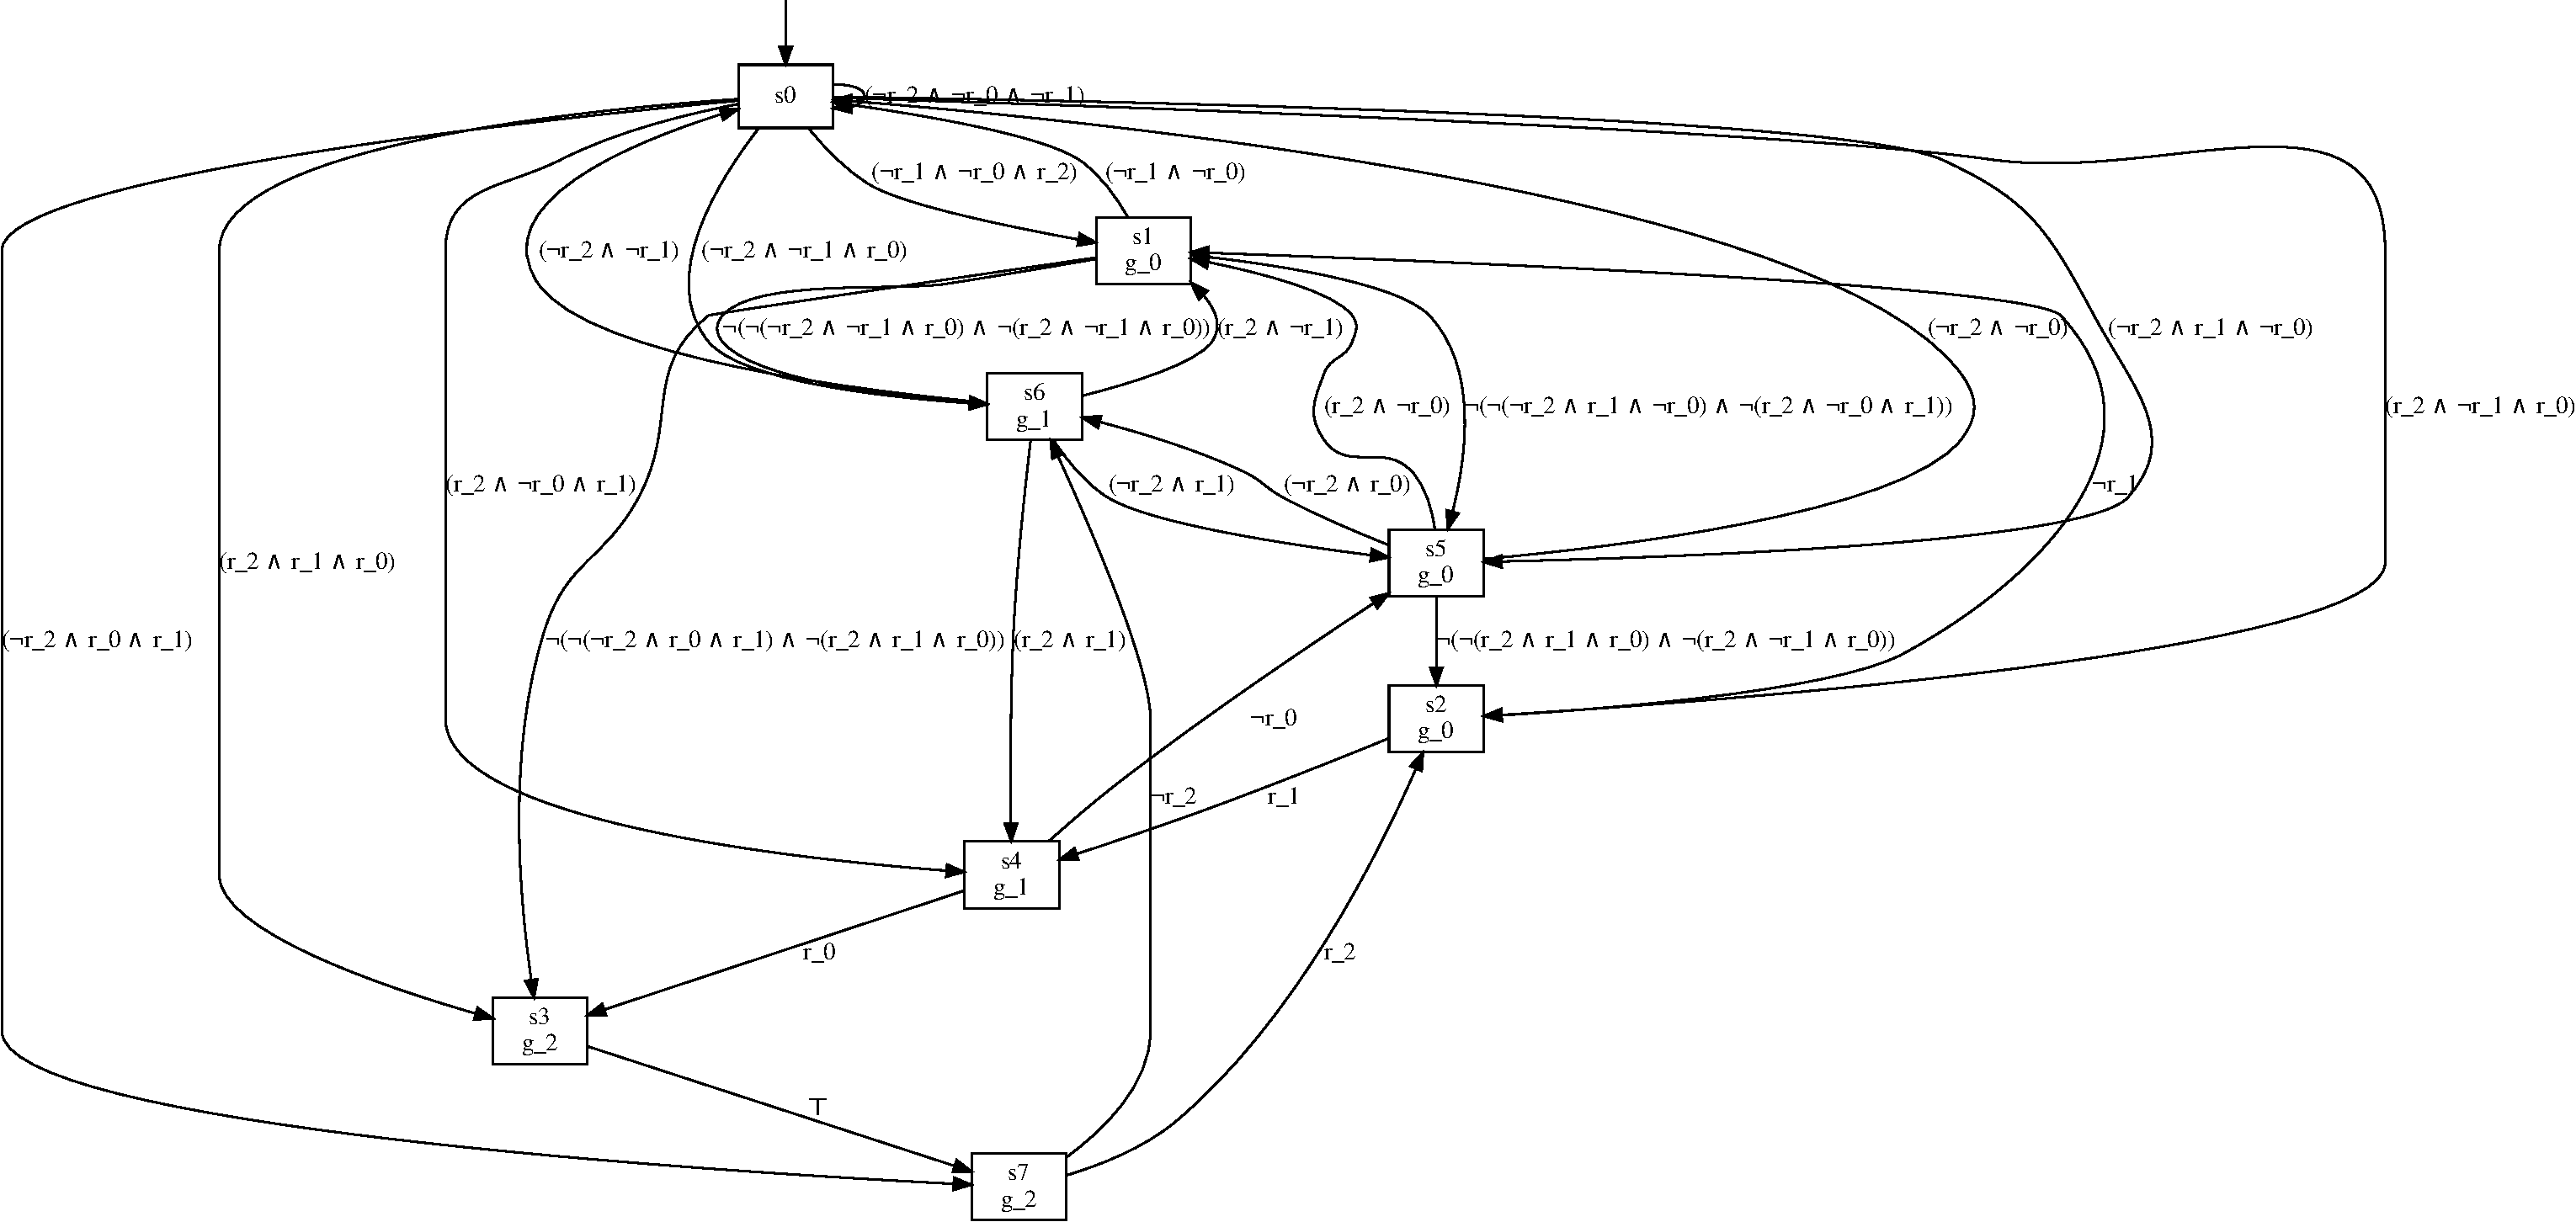
\includegraphics[rotate=90, width=\textwidth, max height=\maxheight{3}-100pt]{images/syntcomp-bosy.pdf}
    \caption{Система переходов $\mathcal{T}_{\text{original}}$, полученная с помощью BoSy для инстанса \texttt{full\_arbiter\_3}: ${C = 8}$ состояний, ${T = 28}$ переходов, суммарный размер охранных условий ${N = 147}$}%
    \label{fig:syntcomp-bosy}
\end{figure}

\begin{figure}[p]
    \centering
    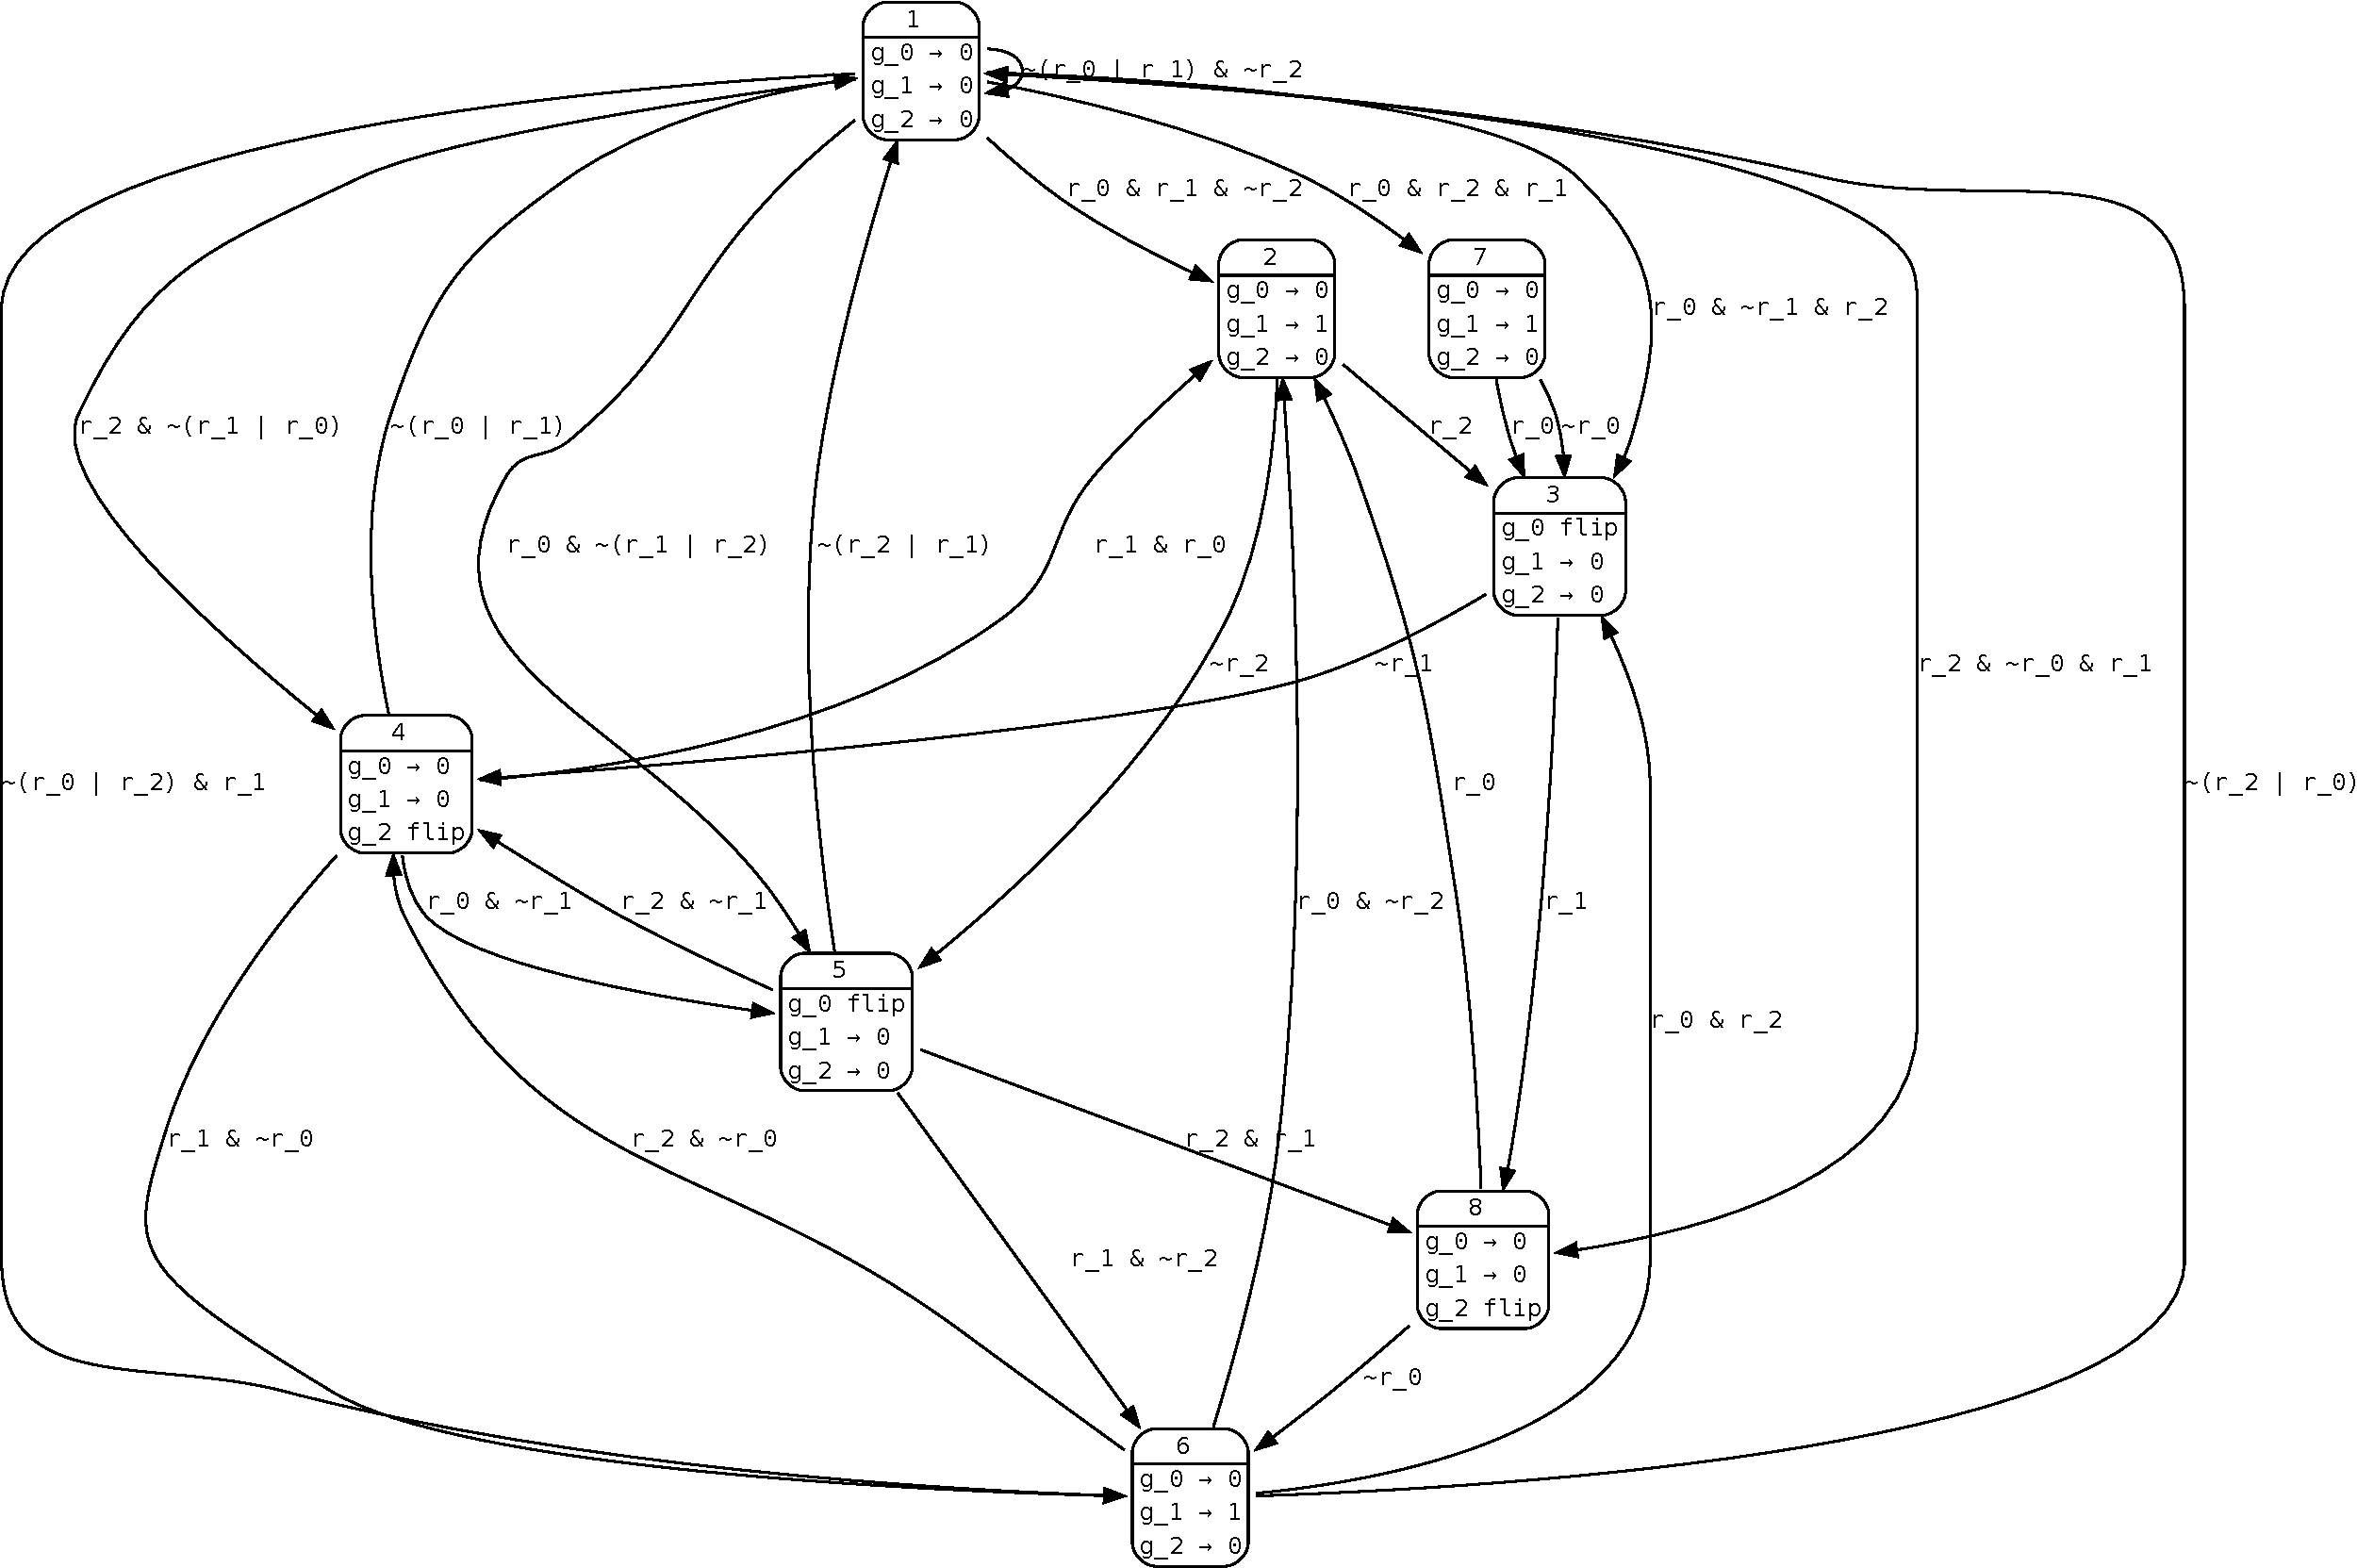
\includegraphics[rotate=90, width=\textwidth, max height=\maxheight{3}]{images/syntcomp-fbsat-deterministic.pdf}
    \caption{Детерминированная минимизированная система переходов $\Automaton_{\text{deterministic}}$, полученная с помощью \smallcaps{fbSAT}, с меньшим суммарными размером охранных условий:~${N = 105}$}%
    \label{fig:syntcomp-fbsat-deterministic}
\end{figure}

\begin{figure}[p]
    \centering
    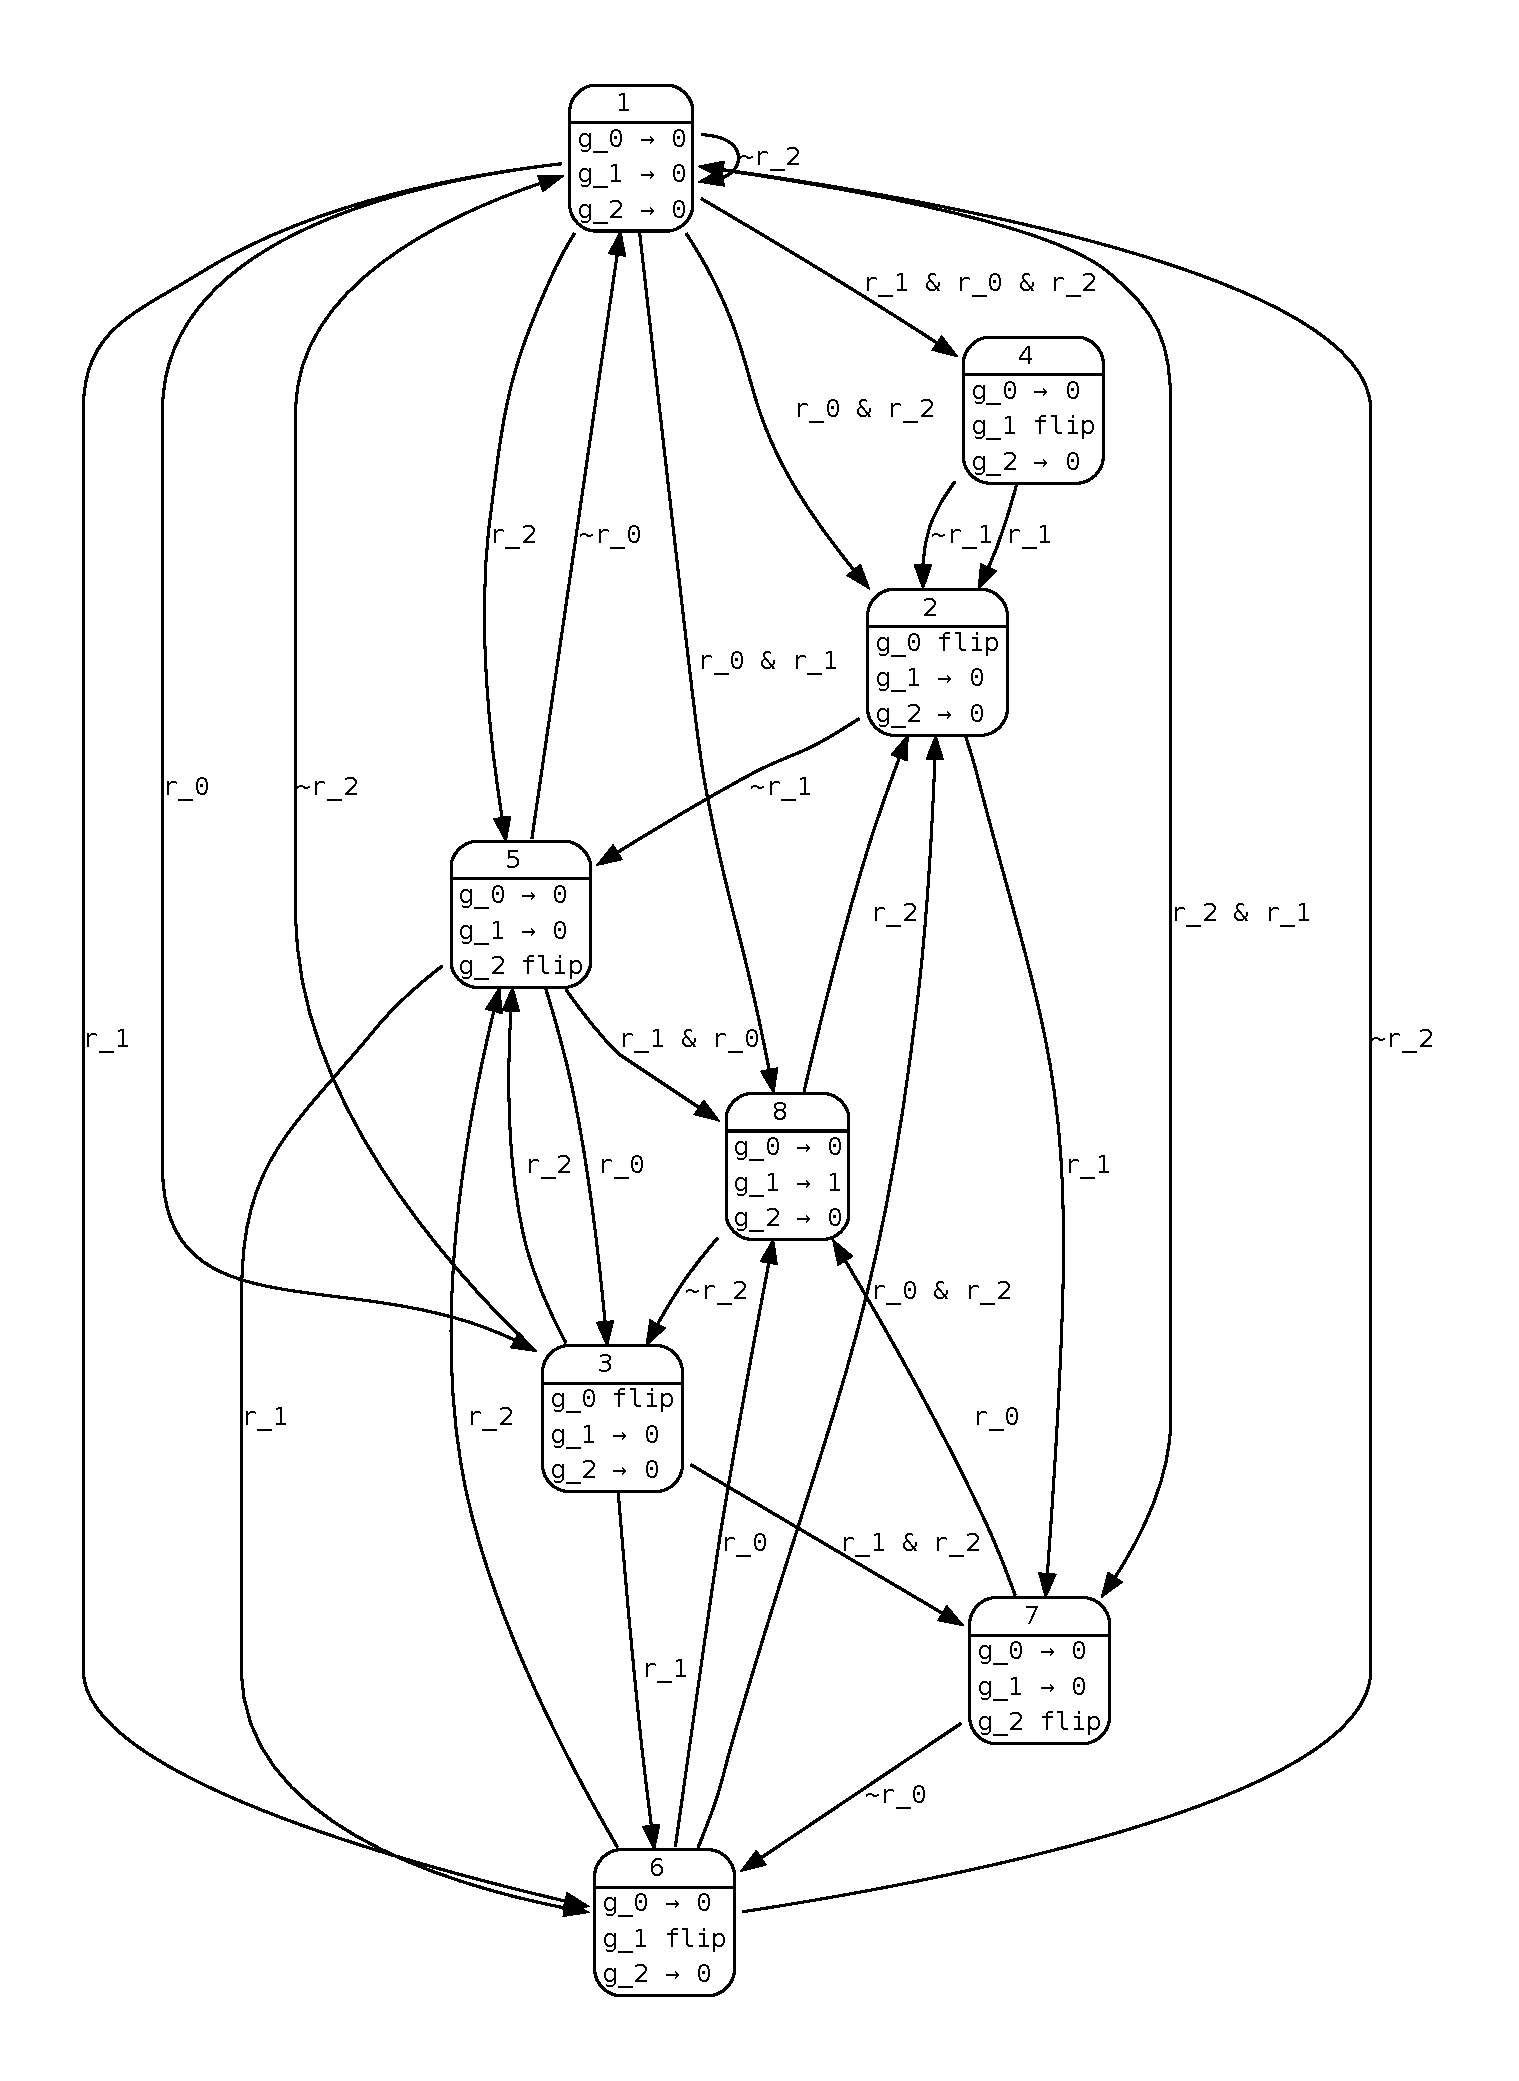
\includegraphics[width=\textwidth, max height=\maxheight{3}]{images/syntcomp-fbsat.pdf}
    \caption{Минимальная недетерминированная система переходов $\Automaton_{\text{non-deterministic}}$, полученная с помощью \smallcaps{fbSAT}, с ещё меньшим суммарным размером охранных условий:~${N = 52}$}%
    \label{fig:syntcomp-fbsat}
\end{figure}


\chapter{Основные публикации автора по теме диссертации}
\label{app:publications}

\newcommand{\mypublication}[2][-]{% [<pages>]{<path>}
    \includepdf[
        pages={#1},
        pagecommand={},  % to include global numbering
        scale=0.9,  % to leave space for the global page numbers
        frame, % (optional)
    ]{#2}
}

\begin{refsection}[biblio/own.bib]
\nocite{
    chivilikhin2020, % PLC
    chukharev2020,   % CEGIS
    chukharev2020b,  % BF
    chukharev2022,   % fbSAT
    semenov2022,     % LEC
    andreev2024      % IMP
}
\printbibliography[
    keyword=own,
    % title={Список всех публикаций автора по теме диссертации},
    % heading=subbibliography,
    heading=none,
    resetnumbers=true
]
\end{refsection}

% \mypublication{biblio/MyPublications/2020_PLC.pdf}
% \mypublication{biblio/MyPublications/2020_CEGIS.pdf}
% \mypublication{biblio/MyPublications/2020_BF.pdf}
% \mypublication{biblio/MyPublications/2022_fbSAT.pdf}
% \mypublication{biblio/MyPublications/2022_LEC.pdf}
% \mypublication{biblio/MyPublications/2024_IMP.pdf}
